In der Einleitung dieser Arbeit wurde bereits h"aufiger vom \emph{Filtern} gesprochen.
Bevor wir uns mit Techniken des Filterns besch"aftigen k"onnen, wollen wir formal festhalten, was unter einem Filter zu verstehen ist.

\begin{defn}[Filter]\label{defn:chap3:filter}
Sei $M$ eine nichtleere Menge. Eine Abbildung der Gestalt
\[
\mathfrak{F}\colon M \to \{0,1\},\ % \text{ mit }
m\mapsto\mathfrak{F}(m)
\]
hei"st \emph{Filterfunktion} oder \emph{Filter auf der Menge $M$}. Die Zuordnung $m\mapsto\mathfrak{F}(m)$ nennen wir das \emph{Filtern von $m$ aus $M$}.
\end{defn}

Damit k"onnen wir uns nun in diesem Kapitel der Frage widmen, ob und wie man aus der Menge aller Eigenpaare eines Eigenwertproblems mit der zugeh"origen Eigenwertgleichung
\[
Ax = \lambda Bx
\]
eine gew"unschte Teilmenge ausw"ahlen kann.
Dabei wollen wir an die Matrizen $A$ und $B$ zun"achst keine weiteren Anforderungen stellen.\\

Ist $M$ entweder die Potenzmenge des Spektrums oder die Menge aller Eigenpaare von $(A,B)$ und $\mathfrak{F}$ eine Filterfunktion auf $M$, so wollen wir vereinbaren, dass wir stets auf der Suche nach der Urbildmenge $\mathfrak{F}^{-1}(\{ 1\})$ sind.
Wollen wir etwa die Menge $G$ aller ganzzahligen Eigenwerte eines Eigenwertproblems finden, so gelte $\mathfrak{F}^{-1}(\{1\}) = G$. In den meisten F"allen werden wir zwar nicht von einer konkreten Filterfunktion der oben definierten Art sprechen, wollen sie aber als latent vorhanden wissen.\\

Die Methoden zur Bestimmung von Teilmengen von Eigenpaaren oder Eigenwerten sind ebenso vielf"altig wie die M"oglichkeiten, das gesamte Spektrum und entsprechende Eigenvektoren zu bestimmen.
Wir wollen aber im Rahmen dieser Arbeit aus dem Katalog der Verfahren lediglich zwei diskutieren: das \emph{Rayleigh-Ritz Verfahren} und die \emph{Konturintegration}.

\newpage

\section{Rayleigh-Ritz Verfahren}\label{sec:chap3:rayleighRitz}
%\footnote{Dieser Abschnitt orientiert sich in Formulierung und Dramaturgie an Abschnitt 4.3.1 aus Y. Saad Solving large evp. Hier verallgemeinern wir aber die Konzepte direkt auf allg. ewp.}
Die Idee dieser Klasse von Verfahren ist die Approximation des von
den gesuchten Eigenvektoren aufgespannten Unterraums.
Bevor wir uns mit beliebigen Eigenwertproblemen $(A,B)$ auseinandersetzen, betrachten wir den Spezialfall $B=I_n$ und wenden uns entsprechend der Eigenwertgleichung
\[
Ax = \lambda x
\]
zu. Sei im Folgenden $\S_m\subseteq\Cn$ ein $m$-dimensionaler Unterraum. Dieser zun"achst nicht
n"aher bestimmte \emph{Suchraum} wird als Grundlage f"ur das Verfahren gew"ahlt.
Gesucht sind nun Paare $(\widetilde{\lambda}, \widetilde{x})\in\C\times (\S_m \setminus\{0\})$,
welche wir als approximierte L"osungen des Eigenproblems verstehen wollen, die
die Eigenschaft
\begin{equation}\label{eq:chap3:orthogonal}
s^H(A\widetilde{x} - \widetilde{\lambda}\widetilde{x})=0
\end{equation}
f"ur alle $s \in \S_m $ erf"ullen. Das \emph{Residuum} $(A\widetilde{x} - \widetilde{\lambda}\widetilde{x})$
soll also orthogonal auf dem Suchraum stehen. Paare, die diesem Anliegen nachkommen,
werden auch \emph{Ritz-Paare von $A$ bez"uglich des Suchraums $\S_m$} genannt.\\

Wir wollen nun annehmen, dass mit der Menge $\{s_i\}_{i=1:m}\subseteq \Cn$ eine Basis orthonormaler Vektoren (ONB) des Unterraums $\S_m$ gegeben ist. Setzen wir dann $S_m :=[s_i]_{i=1:m}\in\C^{n,m}$, so muss wegen $\widetilde{x}\in\S_m$
ein Vektor $y\in\C^m$ mit $S_m y = \widetilde{x}$ existieren. Die Forderung \eqref{eq:chap3:orthogonal}
ist dann zu der Gleichung
\[
S_m^H(AS_m y - \widetilde{\lambda} S_m y) = 0
\]
"aquivalent. Als direkte Konsequenz dieser Umformulierung erhalten wir unter Ausnutzung
der Orthonormalit"at der Spalten von $S_m$ mit
\begin{equation}\label{eq:chap3:transform}
(S_m^H A S_m) y = \widetilde{\lambda}y
\end{equation}
die Eigenwertgleichung zum Eigenwertproblem $(S_m^H A S_m, I_m)$. Jede L"osung $(\widetilde{\lambda},y)$ von \eqref{eq:chap3:transform}
liefert dann nach Konstruktion mit $(\widetilde{\lambda}, S_m y)$ ein Ritz-Paar des gew"ohnlichen
Eigenwertproblems bez"uglich des Suchraums $\S_m$.\\

In Abh"angigkeit von der Wahl
des Suchraumes variiert nat"urlich die G"ute der Approximation. Ist etwa $\S_m$
durch Eigenvektoren aufgespannt, so ist jedes Ritz-Paar schon ein Eigenpaar.
Wir werden sp"ater aus den Untersuchungen des Eigenwertproblems f"ur beliebiges $B$ folgern,
dass bereits im Falle der $A$-Invarianz von $\S_m$ jedes Ritz-Paar von $A$ bez"uglich $\S_m$ bereits ein Eigenpaar von $A$ ist.

\newpage

Die eben skizzierte Vorgehensweise zur Berechnung von Ritz-Paaren des gew"ohnlichen Eigenwertproblems
l"asst sich algorithmisch wie folgt zusammenfassen.

\begin{algorithm}
\caption{Berechnung von Ritz-Paaren (Vgl. \cite[Algorithmus 4.5, S. 98]{saad})}\label{alg:chap3:rp}
\vspace{.15cm}
\textbf{Input:} Matrix $A$ und Suchraum $\S_m$\\
\textbf{Output:} Ritz-Paare von $A$ bzgl. $\S_m$
\begin{algorithmic}[1]
\State Berechne eine ONB $\{s_i\}_{i=1:m}$ von $\S_m$ und setze $S_m\gets[s_i]_{i=1:m}$.
\State Setze $\widetilde{A}\gets S_m^H A S_m$.
\State Finde Eigenpaare von $\widetilde{A}$ und w"ahle die gew"unschten $k$ Paare $(\widetilde{\lambda}_i, y_i)_{i=1:k}$, $k\le m$ aus.
\State Gib Ritz-Paare $(\widetilde{\lambda}_i, S_m y_i)_{i=1:k}$ aus.
\end{algorithmic}
\end{algorithm}

Die Idee dieser Methode ist also simpel: Transformiere das Eigenwertproblem mit
einer gewissen Matrix in ein anderes Eigenwertproblem und benutze dessen L"osungen,
um Ritz-Paare des urspr"unglichen Problems zu erhalten.\\

Doch wozu die M"uhe, das urspr"ungliche Eigenwertproblem in ein anderes
Eigenwertproblem zu "uberf"uhren? Zwar gelingt es, aus dem transformierten Problem
\eqref{eq:chap3:transform} Ritz-Paare zu extrahieren, aber w"are nicht auch denkbar,
s"amtliche Eigenpaare von $A$ zu approximieren und die zum Unterraum $\S_m$
korrespondierende Teilmenge direkt auszuw"ahlen?\\

Dies mag in Einzelf"allen in der Tat sinnvoller sein. Sprechen wir allerdings
von Matrixdimensionen hinreichender Gr"o"se, ist eine vollst"andige
Berechnung aller Eigenpaare mitunter ein sehr zeitintensives Vergn"ugen, wie wir im f"unften Kapitel sehen werden.\\

Bei
genauerer Betrachtung der Gleichung \eqref{eq:chap3:transform} f"allt auf, dass die
Matrix $(S_m^H A S_m) \in \C^{m,m}$ im Falle $n \gg m$ ein deutlich kleineres
Format hat als die Matrix $A$ im urspr"unglichen Problem. Man darf hier also erwarten,
dass die ben"otigte Laufzeit zur Bestimmung der Ritz-Paare mit dem Algorithmus \ref{alg:chap3:rp}
geringer ist als beim Approximieren s"amtlicher Eigenpaare von $A$. Auch das
wird im f"unften Kapitel anhand ausgew"ahlter Beispiele vorgef"uhrt.\\

Nun, da wir uns mit der Idee der Rayleigh-Ritz Methode vertraut gemacht haben, erweitern wir die obige Theorie auf Probleme der Art $(A,B)$ f"ur beliebiges $B$ und betrachten entsprechend die Eigenwertgleichung
\begin{equation}\label{eq:chap3:gevp}
Ax = \lambda Bx.
\end{equation}
Dabei gehen wir ganz analog zum gew"ohnlichen Eigenwertproblem vor und betrachten wieder
einen $m$-dimensionalen Suchraum $\S_m\subseteq \Cn$.
Gefunden werden sollen dieses Mal Paare $ (\widetilde{\lambda}, \widetilde{x}) \in \C
\times (\S_m \setminus\{ 0\})$, die der Orthogonalit"atsbedingung
\begin{equation}\label{eq:chap3:borthogonal}
A\widetilde{x} - \widetilde{\lambda}B\widetilde{x} \ \bot \ \S_m
\end{equation}
gen"ugen.

\newpage

Durch die Wahl eines geeigneten Vektors $y\in\C^m$ kann die N"aherungsl"osung $\widetilde{x}$ wie zuvor durch das Produkt $S_m y$ ersetzt werden, wobei die Spalten von $S_m$ erneut eine ONB des Suchraums $\S_m$ bilden.
Damit l"asst sich die zu \eqref{eq:chap3:borthogonal} "aquivalente Forderung
\[
S_m^H(AS_m y - \widetilde{\lambda} BS_m y) = 0.
\]
aufstellen. Wie bereits beim gew"ohnlichen Eigenwertproblem l"asst sich nun aus jeder L"osung
$(\widetilde{\lambda}, y)$ von
\begin{equation}\label{eq:chap3:transformedevp}
(S_m^H AS_m) y = \widetilde{\lambda} (S_m^H B S_m) y.
\end{equation}
mit $(\widetilde{\lambda}, S_m y)$ ein Ritz-Paar f"ur das Eigenwertproblem $(A,B)$ gewinnen.\\

Da mit der Matrix $B$ ein weiterer Darsteller ber"ucksichtigt werden muss, zieht dies als Konsequenz eine Anpassung des Algorithmus \ref{alg:chap3:rp} nach sich. Wir k"onnen diesen in der folgenden Manier abwandeln.

\begin{algorithm}
\caption{Berechnung von Ritz-Paaren}\label{alg:chap3:grp}
\vspace{.15cm}
\textbf{Input:} Matrizen $A,B$ und Suchraum $\S_m$\\
\textbf{Output:} Ritzpaare von $(A,B)$ bzgl. $\S_m$
\begin{algorithmic}[1]
\State Berechne ONB $\{s_i\}_{i=1:m}$ von $\mathcal{S}_m$ und setze $S_m\gets[s_i]_{i=1:m}$.
\State Setze $\widetilde{A}\gets S_m^H A S_m$,
$\widetilde{B} \gets S_m^H BS_m$.
\State Finde Eigenpaare von $(\widetilde{A},\widetilde{B})$ und w"ahle die gew"unschten $k$ Paare $(\widetilde{\lambda}_i,y_i)_{i=1:k}$ f"ur $k\le m$ aus.
\State Gib Ritz-Paare $(\widetilde{\lambda}_i, S_m y_i)_{i=1:k}$ aus.
\end{algorithmic}
\end{algorithm}

Bei den beiden vorgestellten Algorithmen ist anzumerken, dass zun"achst nicht von einer Eigenpaarfilterung im Sinne der Definition \ref{defn:chap3:filter} geprochen werden kann.
Schlie"slich erhalten wir unter Umst"anden kein exaktes Eigenpaar, sondern eben nur einen Ersatz.
Um eine zufriedenstellende Qualit"at dieses Ersatzes gew"ahrleisten zu k"onnen, ist es erforderlich, die Wahl des Suchraums nicht dem Geschick alleine zu "uberlassen, sondern eine gegebenenfalls weniger geschickte Wahl algorithmisch kompensieren zu k"onnen.\\

Dies kann zum Beispiel durch das Einf"uhren einer Iterationsvorschrift gelingen, die den Suchraum in jedem Iterationsschritt "andert.
Damit lassen sich zu ber"ucksichtigende Toleranzen, beispielsweise eine maximale euklidische Abweichung der Ritz-Werte zu den Eigenwerten oder Vorgaben bez"uglich des Winkels zwischen Eigenraum und dem Unterraum der Ritz-Vektoren, einhalten.
Wir werden diese Idee zu einem sp"ateren Zeitpunkt in dieser Arbeit weiterverfolgen.\\

Wir wollen uns nun vorerst von der Algorithmik verabschieden und einige Beobachtungen
festhalten. Es wurde behauptet, dass die Invarianz des Suchraumes $\S_m$ unter
$A$ dazu f"uhrt, dass jedes Ritz-Paar bez"uglich $\S_m$ ein Eigenpaar von $A$ ist.
Doch warum ist das so? Dies zu beantworten verpflichtet sich der folgende Satz.

\newpage

\begin{thm}\label{thm:chap3:invariant}
Neben zwei Matrizen $A,B\in\Cnn$ -- wobei wir Hermitizit"at und positive Definitheit von $B$ fordern -- sei ein $m$-dimensionaler Unterraum $\S_m \subseteq \C^n$ gegeben.
Ist dieser invariant unter $B^{-1}A$, so ist jedes Ritz-Paar von $B^{-1}A$
bez"uglich $\S_m$ auch ein Eigenpaar von $(A,B)$.
\end{thm}

\begin{proof}
Beginnen wir mit einer ONB $\{s_i\}_{i=1:m}\subseteq\S_m$ des Unterraums $\S_m$
und setzen wie bisher $S_m := [s_i]_{i=1:m}\in\C^{n,m}$. Aufgrund der Invarianz
von $\S_m$ unter $B^{-1}A$ muss eine Matrix $V_m \in \C^{m,m}$ existieren, welche
die Gleichung
\begin{equation}\label{eq:chap3:thminvariant}
B^{-1}A S_m = S_m V_m
\end{equation}
erf"ullt. Insbesondere folgt unter Ausnutzung der Orthonormalit"at der Spalten
von $S_m$ die Identit"at $S_m^H B^{-1}A S_m = V_m$.
Sind nun $\lambda\in\C$ und $y\in\C^m\setminus\{0\}$ so gew"ahlt, dass $(\lambda, S_m y)$
ein Ritz-Paar von $B^{-1}A$ bez"uglich $\S_m$ ist, so ist $(\lambda, y)$ ein Eigenpaar von $V_m$. Es folgt daher
mit \eqref{eq:chap3:thminvariant} die Gleichung
\[
B^{-1}AS_m y = S_m V_m y = \lambda S_m y
\]
und schlie"slich auch die Behauptung durch Umstellen.
\end{proof}

Aus dem eben bewiesenen Resultat k"onnen wir nun f"ur das gew"ohnliche Eigenwertproblem unmittelbar das folgende Korollar
ableiten.

\begin{kor}
Ist $A\in\Cnn$ und $\S_m\subseteq \Cn$ ein $m$-dimensionaler $A$-invarianter Unterraum, so ist
jedes Ritz-Paar von $A$ bez"uglich $\S_m$ ein Eigenpaar von $A$.
\end{kor}

\begin{proof}
Betrachte f"ur $B:=I_n$ das Eigenwertproblem $(A,B)$
mit der zugeh"origen Eigenwertgleichung
\[
Ax = \lambda Bx = \lambda x.
\]
Die Aussage folgt dann aus dem vorigen Satz.
\end{proof}

Wenden wir uns einem weiteren Resultat zu. Zwischen dem Rayleigh-Ritz Verfahren und dem Konzept der Projektion besteht ein enger Zusammenhang.
Um zu dieser Einsicht zu gelangen, bedarf es ein wenig
Vorbereitung.
%Das Rayleigh-Ritz-Verfahren steht in einem engen Zusammenhang zu Projektionsverfahren.
%Mit einer geeigneten Projektionsmatrix $P\in\Cnn$ ist ein Paar $(\lambda, x)\in\C\times\Co$
%\textcolor{red}{(oder $\in\C\times\U_m\setminus\{0\}$?)} genau dann eine L"osung
%der Gleichung \eqref{chap2:gevp}, wenn es eine L"osung von
%\[
%P^H APx = \lambda P^H BPx
%\]
%ist. Richtig definiert, besitzt $P$ noch weitere n"utzliche Eigenschaften, die
%der folgende Satz vorstellt.
\begin{thm}\label{thm:chap3:projektor}
Es sei $B\in\Cnn$ eine HPD-Matrix und $\S_m \subseteq \Cn$ ein $m$-dimensionaler Unterraum. Sei weiter $\{s_i\}_{i=1:m}\subseteq\S_m$ eine
Basis $B$-orthonormaler Vektoren, das hei"st, die Matrix $S_m := [s_i]_{i=1:m}
\in\C^{n,m}$ erf"ulle die Gleichung $S_m^H B S_m = I_m$. Dann ist die von der Matrix
 $P := S_m S_m^H B \in \Cnn$ induzierte lineare Abbildung
\[
p \colon \Cn \to \Cn, x\mapsto S_m S_m^H Bx
\]
eine $B$-orthogonale Projektion auf den Unterraum $\S_m$. Au"serdem gilt
f"ur alle $x\in\Cn$ die Identit"at
\[
\|x-p(x)\|_B = \min_{y\in\S_m} \|x - y\|_B.
\]
\end{thm}

\newpage

\begin{proof}
Nach Konstruktion gilt $p(\Cn)\subseteq \S_m$. Aus der $B$-Orthogonalit"at von $S_m$ folgt f"ur alle $x\in\Cn$
\[
p^2 (x) = S_m S_m^H B S_m S_m^H B x= S_m S_m^H Bx = p(x).
\]
%und damit gilt die Mengengleichheit $p(\Cn) = \U$ nach Konstruktion. %($\Rang{P_B} = \dim(\U)$).
Ist nun $x\in\Cn$ vorgegeben, dann folgt unter erneuter Ausnutzung von $S_m^H BS_m = I_m$
\[
S^H B (x-p(x)) = S^H B (I_n - S_m S_m^H B)x
=(S^H B - S^H B S S^H B)x = 0
\]
und somit $x-p(x) \perp_B \S_m$. Damit ist gezeigt, dass $p$ eine $B$-orthogonale Projektion auf $\S_m$ ist. Die Optimierungsaufgabe wird schlie"slich wegen
\begin{align*}
\|x-y\|_B^2 &= \|x-p(x) + p(x)-y\|_B^2 \\
&= \|x-p(x)\|_B^2 + \|p(x)-y\|_B^2\\
&\ge \|x-p(x)\|_B^2
\end{align*}
gel"ost. Dabei ist bei der zweiten Gleichheit zu ber"ucksichtigen, dass $x-p(x) \in \S_m^{\bot_B}$
und $p(x)-y \in \S_m$ gilt.
\end{proof}

Mit Hilfe der im Satz eingef"uhrten Projektionsmatrix $P$ l"asst sich die Gleichung
\eqref{eq:chap3:transformedevp} umformulieren. Durch Linksmultiplikation
mit $B^H S_m$ und dem Einschub der Identit"at $S_m^H B S_m$ gilt n"amlich
\[
B^H S_m (S_m^H A S_m)(S_m^H B S_m)y = \widetilde{\lambda} B^H S_m (S_m^H B S_m)(S_m^H B S_m)y
\]
und folglich
\[
P^H A P S_m y = \widetilde{\lambda} P^H B P S_m y.
\]
Wenn wir uns an dieser Stelle erinnern, dass $\widetilde{x}$ durch $S_m y$ ersetzt wurde, so
erhalten wir
\[
P^H A P \widetilde{x} = \widetilde{\lambda} P^H B P \widetilde{x}.
\]
Im Fall der gew"ohnlichen Eigenwertgleichung erhalten wir speziell
\[
P^H A P \widetilde{x} = P A P \widetilde{x} = \widetilde{\lambda} \widetilde{x}.
\]

Die Behauptung, es w"urde ein Zusammenhang zu Projektionen bestehen, wurde also in der Tat zu Recht aufgestellt.\\

Nach diesen theoretischen Ausf"uhrungen fragt sich der anwendungsorientierte Leser zu Recht, welcher Nutzen aus den obigen Einsichten gezogen werden kann.
Daf"ur wenden wir uns erneut dem Rayleigh-Ritz Verfahren zu und betrachten nun den Spezialfall eines hermitesch positiv definiten Eigenwertproblems $(A,B)$.

\newpage

Angenommen, uns st"unde mit dem Suchraum $\S_m$ bereits ein von Eigenvektoren
aufgespannter Unterraum zur Verf"ugung. Dann sichert uns Satz \ref{thm:chap2:realEigenvalues} die Existenz einer Matrix $S_m := [s_i]_{i=1:m}\in\C^{n,m}$ mit
$B$-orthonormalen Spalten aus Eigenvektoren von $(A,B)$ und $\Bild(S_m)=\S_m$, sowie die Existenz einer reellen Diagonalmatrix
$\Lambda_m := \text{diag}(\lambda_i)_{i=1:m}\in\R^{m,m}$ mit
\[
AS_m = BS_m\Lambda_m.
\]
Dabei entsprechen die Diagonaleintr"age von $\Lambda_m$ gerade den zu den Spalten
von $S_m$ korrespondierenden Eigenwerten von $(A,B)$. Folglich w"are das Bild
des Spektralprojektors $P=S_m S_m^H B$ nach Konstruktion wegen
\[
B^{-1}AP = B^{-1}(AS_m)S_m^H B = B^{-1}(BS_m \Lambda)S_m^H B
= S_m\Lambda S_m^H B = \left(\sum_{i=1}^m \lambda_i s_i s_i^H\right)\cdot B
\]
ein $(B^{-1}A)$-invarianter Unterraum. Daher erscheint es
wegen Satz \ref{thm:chap3:invariant} sinnvoll, den Spektralprojektor $P$ in das
Rayleigh-Ritz-Verfahren zu integrieren.
Da jedoch der Unterraum $\S_m$ im Allgemeinen nicht bekannt ist, stellt sich die Frage, ob es
"uberhaupt sinnvoll ist nach dem Projektor zu suchen.
Wir werden jedoch alsbald feststellen, dass %zumindest
die Matrix $S_m S_m^H$ mit Methoden der Funktionentheorie berechenbar ist.

\section{Konturintegration}\label{sec:chap3:konturintegration}

Betrachten wir ein $n$-dimensionales Eigenwertproblem $(A,B)$. Zu einer gegebenen Teilmenge $\Lambda_1$ vom Spektrum dieses Problems wollen wir
den Spektralprojektor $P_1$ konstruieren, welcher Vektoren auf den von den zu $\Lambda_1$ korrespondierenden Eigenvektoren aufgespannten Unterraum $\S_1$ projiziert.
Dazu schr"anken wir uns vorerst auf das gew"ohnliche Eigenwertproblem $(A,I_n)$ ein und orientieren
%/präsentieren in den folgenden zeilen die Gedankengänge aus ...
uns in
den folgenden Ausf"uhrungen an der Herleitung von \cite[Abschnitt 4.9]{liesen}.
Dabei nehmen wir uns die Freiheit, die Notation an die hiesige Arbeit anzupassen und gelegentlich von den vorgeschlagenen Schreibweisen abzuweichen.\\

Wir wollen annehmen, dass die Zahl $m$ der Dimension von $\S_1$ entspricht. Seien Matrizen $A_1\in\C^{m,m},
A_2\in\C^{n-m,n-m}$ und $S\in\Cnn$ derart vorgegeben, dass  $\Lambda(A_1) = \Lambda_1$ einerseits und $\Lambda_2 := \Lambda(A_2)$ mit $\Lambda_2 \cap \Lambda_1 = \emptyset$ andererseits gelten und eine Faktorisierung der Art
\begin{equation}\label{eq:chap3:factorization}
A = S\begin{bmatrix} A_1 & 0 \\ 0 & A_2 \end{bmatrix} S^{-1}
\end{equation}
existiert.\footnote{Diese Zerlegung kann beispielsweise mit Hilfe der Jordan'schen Normalform erreicht werden.}
Dann k"onnen wir zwei Matrizen $S_1 \in \C^{n,m}$ mit $\Bild(S_1) = \S_1$ und
$S_2 \in \C^{n,n-m}$ finden, welche die Partionierung $S=[S_1, S_2]$ erlauben.

\newpage
%Wir werden zu einem sp"ateren Zeitpunkt untersuchen, inwieweit die Numerik in der Lage ist, dieses Verfahren algorithmisch umzusetzen. Im Folgenden betrachten wir stets das HPD-Eigenwertproblem $(A,B)$.\\
Durch Definition der Matrix
\begin{equation}\label{eq:chap3:projection}
P_1 := S \begin{bmatrix} I_m & 0 \\ 0 & 0 \end{bmatrix}S^{-1}
\end{equation}

erhalten wir dann eine Projektion auf $\S_1$: Nach Konstruktion gilt $P_1 x \in \S_1$ f"ur alle $x\in\Cn$
und $P_1^2 = P_1$. Andererseits liefert die Matrix
\[
P_2 := I_n - P_1
\]
eine Projektion auf $\S_2 := \Bild(S_2)$: Es gilt $P_2 x\in\S_2$ f"ur alle $x\in\Cn$ und
\[
P_2^2 = (I_n - P_1)^2 = I_n - 2P_1 + P_1^2 = I_n - P_1.
\]
Da sich jeder Vektor $x\in\Cn$ in
\[
x = P_1 x + (I_n - P_1)x
\]
dekomponieren l"asst und trivialerweise $P_2 x \bot \S_2^\bot$ gilt, k"onnen wir schlie"sen, dass $P_1$ orthogonal bez"uglich $\S_2^\bot$ auf $\S_1$ abbildet.\\

Der Projektor $P_1$ aus \eqref{eq:chap3:projection} l"asst sich mit Hilfe eines Integrals darstellen. Bevor wir dazu kommen, ben"otigen wir zus"atzliches Vokabular.

\begin{defn}[Jordan-Kurve]\label{defn:chap3:jordanKurve}
Es sei $\gamma\colon\{x\in\R^2 : \|x\|_2 = 1\}\to\R^2$ eine Abbildung, die hom"oomorph auf ihr Bild abbildet.
Dann hei"st $\Gamma := \Bild(\gamma)$ \emph{Jordan-Kurve}.
\end{defn}

\begin{figure}[h!]\label{im:chap3:jKurve}
\center
\begin{subfigure}[c]{.3\textwidth}
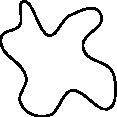
\includegraphics[width=.9\linewidth]{images/jKurve}
\subcaption{Jordan-Kurve.}
\end{subfigure}
\qquad
\begin{subfigure}[c]{.3\textwidth}

\includegraphics[width=.9\linewidth]{images/nJKurve}
\subcaption{Keine Jordan-Kurve.}
\end{subfigure}
\caption{Skizze zweier Kurven.}
\end{figure}

Insbesondere sind Jordan-Kurven also geschlossene und "uberschneidungsfreie Kurven.\\

Da wir "uber solche Jordan-Kurven integrieren wollen, f"uhren wir noch den Begriff der \emph{orientierten Kurve} ein.
Dabei wollen wir es jedoch der Einfachheit halber bei einer informellen Beschreibung belassen.
Eine Jordan-Kurve hei"st \emph{positiv orientiert},
falls sie in ihrer Parametrisierung im mathematisch positiven Sinne \glqq durchlaufen\grqq\ wird (Vgl. Abb. \ref{im:chap3:jKurveOrientiert}).

\newpage

\begin{figure}[h!]
\center
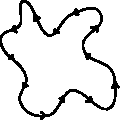
\includegraphics[width=.27\linewidth]{images/jKurveOrientiert}
\caption{Skizze einer positiv orientierten Jordan-Kurve.}\label{im:chap3:jKurveOrientiert}
\end{figure}



%Zun"achst ist es erforderlich einige Begriffe und Notationen einzuf"uhren. F"ur zwei Zahlen $z_1, z_2 \in\C$ sei mit der Menge
%\[
%[z_1, z_2] := \{(1-t)z_1 + tz_2 \in\C \mid t\in[0,1]\}
%\]
%die direkte Verbindungsstrecke zwischen $z_1$ und $z_2$ bezeichnet. Im Spezialfall $z_1,z_2 \in\R$
%stellen wir uns daher unter $[z_1,z_2]$ ein reellwertiges Intervall eingebettet in die komplexe Zahlenebene vor.
%Des Weiteren ben"otigen wir sogenannte \emph{Jordan-Kurven}. Diese definieren wir im Kontext
%dieser Arbeit wie folgt.

Wir k"onnen nun den Gedanken aus \cite[Abschnitt 4.9]{liesen} weiter folgen und betrachten f"ur $\Omega\subseteq\Cn$ die durch
\[
G\colon\Omega \setminus \Lambda(A) \to\Cnn
\text{, }
t \mapsto (t I_n - A)^{-1}
\]
definierte \emph{Resolventenfunktion} -- auch \emph{Green-Funktion} genannt (Vgl. \cite{polizzi}).
Angenommen, die Menge $\Lambda_1$ liegt im Inneren eines von einer positiv orientierten Jordan-Kurve $\Gamma$ umschlossenen
Gebiets und $\Lambda_2$ im Inneren des Komplementes dieses Gebiets.\footnote{Man beachte, dass im Folgenden stillschweigend die Identifikation $\R^2\cong\C$ benutzt wird.}
Dann gilt die Identit"at
\begin{equation}\label{eq:chap3:kontur}
P_1 = \frac{1}{2\pi\iota}\int_\Gamma G(t)\text{ d}t
\end{equation}
beziehungsweise unter Ausnutzung der Faktorisierung \eqref{eq:chap3:factorization}
\begin{equation}\label{eq:chap3:konturMatrix}
P_1 = \frac{1}{2\pi\iota} S
\begin{bmatrix}
\int_\Gamma (t I_m - A_1)^{-1} \text{ d}t & 0 \\
0 & \int_\Gamma (t I_{n-m} - A_2)^{-1} \text{ d}t
\end{bmatrix} S^{-1}.
\end{equation}

Hierbei ist das Integral eintragsweise zu verstehen und $\iota$ als imagin"are Einheit zu lesen.
Da die Menge $\Lambda_2$ nach Vorgabe au"serhalb des umrandeten Gebietes liegt, folgt aus dem Cauchy'schen Integralsatz\footnote{Siehe Satz \ref{thm:appTheorems:Cauchy} im Anhang \ref{appTheorems}.}
\[
\int_\Gamma (t I_{n-m} - A_2)^{-1} \text{ d}t = 0_{n-m}.
\]
Um die Begr"undung, dass die Gleichheit \eqref{eq:chap3:konturMatrix} korrekt ist, fortsetzen zu k"onnen, ben"otigen wir die folgende Erkenntnis.

\begin{thm}\label{thm:chap3:potenzreihe}
Ist $M\in\Cnn$ mit $\|M\|_2 < 1$, so ist $I_n - M$ invertierbar und es gilt
\[
(I_n - M)^{-1} = \sum_{j=0}^\infty M^j
\]
\end{thm}

\textit{Beweis (Vgl. \cite[Abschnitt 2.3.4]{loan}).}
Zun"achst zur Regularit"at: Angenommen, die Matrix $I_n-M$ w"are nicht invertierbar. Dann muss ein von Null verschiedener Vektor $x\in\Cn$ existieren, mit $(I_n-M)x = 0$.
Wir erhalten insbesondere $x = Mx$. Da die induzierte $2$-Norm f"ur Matrizen bekannterma"sen submultiplikativ ist, gilt $\|x\|_2 \le \|M\|_2\|x\|_2$. Dann f"uhrt aber die Konsequenz $\|M\|_2 \ge 1$ zum Widerspruch.

\newpage

Nun zur Potenzreihenentwicklung: Nutzen wir erneut die Submultiplikativit"at der $2$-Norm, so erhalten wir f"ur alle $k\in\N$ die Absch"atzung $\|M^k\|_2 \le \|M\|_2^k$. Wegen $\|M\|_2 <1$ existiert daher der Grenzwert
\[
\lim_{k\to\infty} M^k = 0_n.
\]
Schlie"slich folgt die Behauptung des Satzes aus
\[
\sum_{j=0}^\infty M^j (I_n-M) =
\lim_{k\to\infty}\sum_{j=0}^k M^j (I_n-M) =
\lim_{k\to\infty} I_n-M^{k+1} = I_n
\]
durch einfaches Umstellen. \hfill $\qed$

\begin{kor}\label{kor:chap3:potenzreihe}
Mit den obigen Notationen folgt f"ur alle $t\in\C$ mit $|t| > \|A_1\|_2$ die Identit"at
\[
(t I_m - A_1)^{-1} = \frac{1}{t} \sum_{j=0}^\infty (t^{-1} A_1)^j.
\]
\end{kor}
\begin{proof}
Man mache sich die Identit"at
\[
(t I_m - A_1)^{-1} = \frac{1}{t}(I_m - t^{-1}A_1)^{-1}
\]
klar und benutze den Satz \ref{thm:chap3:potenzreihe}.
\end{proof}

Wenden wir uns nun wieder der Gleichung \eqref{eq:chap3:konturMatrix} zu. Es bleibt zu zeigen, dass
\begin{equation}\label{eq:chap3:identitaet}
\frac{1}{2\pi\iota}\int_\Gamma (t I_m - A_1)^{-1} \text{ d}t = I_m
\end{equation}
gilt. Dazu halten wir uns nach wie vor an die Ausf"uhrungen von \cite[Abschnitt 4.9]{liesen}. Wie von den Autoren vorgeschlagen, setzen wir
\[
F(A_1,t) := \frac{1}{t}\sum_{j=1}^\infty(t^{-1}A_1)^j
\]
und erhalten mit Hilfe des Korollars \ref{kor:chap3:potenzreihe}
\begin{equation}\label{eq:chap3:resolventenZerlegung}
(t I_m - A_1)^{-1} = \frac{1}{t} I_m + F(A_1,t).
\end{equation}
Nach Konstruktion sind alle Eigenwerte von $A_1$ beziehungsweise die Singularit"aten von $(t I_m - A_1)^{-1}$ im Inneren des von $\Gamma$ umschlossenen Gebiets. Auf der linken Seite von Gleichung \eqref{eq:chap3:identitaet} "andert sich der Wert des Integrals nicht, wenn wir anstelle von $\Gamma$ "uber eine
andere Jordan-Kurve, die das von $\Gamma$ umschlossene Gebiet enth"alt, integrieren. Daher k"onnen wir als Integrationskontur  $\widehat{\Gamma}$ ebenso gut den Kreis um den Nullpunkt mit hinreichend gro"sem Radius $r > \|A_1\|_2$
w"ahlen.

\newpage

F"ur $t\in[0,2\pi]$ ist die Abbildung $t\mapsto re^{\iota t}$ eine Parametrisierung von $\widehat{\Gamma}$. Diese Kurve ist dann positiv orientiert und wir erhalten wegen
\[
\int_{\widehat{\Gamma}} \frac{1}{t} \text{ d}t = \int_0^{2\pi}\frac{1}{r e^{\iota t}} \iota r e^{\iota t} \text{ d}t = 2\pi \iota
\]
und unter Ausnutzung von Gleichung \eqref{eq:chap3:resolventenZerlegung}
\[
\int_\Gamma (t I_m - A_1)^{-1} \text{ d}t =
\int_{\widehat{\Gamma}} \frac{1}{t}I_m
\text{ d}t
+ \int_{\widehat{\Gamma}} F(A_1,t) \text{ d}t
= 2\pi\iota \cdot I_m + \int_{\widehat{\Gamma}} F(A_1,t) \text{ d}t.
\]
Betrachten wir nun f"ur $t \in\widehat{\Gamma}$ den Ausdruck $F(A_1,t)$ etwas genauer.
Es gilt
\[
\|F(A_1,t)\|_2 =
\left\| \frac{1}{t} \sum_{j=1}^\infty \left( \frac{1}{t} A_1 \right)^j \right\|_2
\le \frac{1}{|t|} \sum_{j=1}^\infty \left(\frac{\|A_1\|_2}{|t|} \right)^j
= \frac{\|A_1\|_2}{|t|^2}\sum_{j=0}^\infty \left(\frac{\|A_1\|_2}{|t|} \right)^j.
\]
Nach Konstruktion gilt $\|A_1\|_2 < r \le |t|$.
Mit der Kenntnis "uber den Grenzwert der geometrischen Reihe erhalten wir daher die Absch"atzung
\[
\|F(A_1,t)\|_2 \le \frac{\| A_1 \|_2}{r}
\frac{1}{1-\|A_1\|_2 / r}.
\]
Da diese Absch"atzung f"ur alle $r > \|A_1\|$ gilt und die rechte Seite f"ur $r\to\infty$ den Wert Null annimmt, muss daher
\[
\frac{1}{2\pi\iota}\int_\Gamma (t I_m - A_1)^{-1} \text{ d}t =
 \frac{1}{2\pi\iota} \left(2\pi\iota \cdot I_m + \int_{\widehat{\Gamma}} F(A_1,t) \text{ d}t\right)
= I_m
\]
und somit auch Gleichung \eqref{eq:chap3:kontur} gelten.\\

Welche Schlussfolgerungen lassen sich hieraus f"ur ein Eigenwertproblem $(A,B)$ ziehen, bei der eine beliebige Matrix $B$ vorgegeben ist? Diese Frage soll zumindest f"ur HPD-Eigenwertprobleme beantwortet werden.\\

Sei also $(A,B)$ ein HPD-Eigenwertproblem. Dann ist $B$ invertierbar und jede Singularit"at der Greenfunktion $G_1(t) := (t I_n - B^{-1}A)^{-1}$
ist auch eine Singularit"at der Funktion $G_2(t):=(t B - A)^{-1}$. Ist wie eben $\Lambda_1$ eine Teilmenge des Spektrums, $\Gamma$ eine umschlie"sende Jordan-Kurve und die Zerlegung
\[
B^{-1}A = S\begin{bmatrix} (B^{-1} A)_1 & 0 \\ 0 & (B^{-1} A)_2 \end{bmatrix} S^{-1}
\]
analog zu Gleichung \ref{eq:chap3:factorization} gegeben, so schlie"st man auf "ahnliche Weise
\[
\frac{1}{2\pi\iota}\int_\Gamma (t I_n - B^{-1}A)^{-1} \text{ d}t =
\frac{1}{2\pi\iota}\int_\Gamma (t B - A)^{-1} \text{ d}t
= P_1
\]
f"ur eine entsprechende Matrix $P_1$.
%\section{Zusammenfassung}

%An dieser Stelle wollen wir kurz zusammentragen, was bisher diskutiert wurde und identifizieren, wie die in den vorigen Abschnitten besprochenen Konzepte mit dem Filtern zusammenh"angen. Sei dazu im Folgenden mit $(A,B)$ ein Eigenwertproblem gegeben.\\

%Das zentrale Thema des Abschnittes \ref{sec:chap3:rayleighRitz} war das Rayleigh-Ritz Verfahren. Hierbei wurden ausgehend von einem Suchraum Ritz-Paare gesucht, die einer gewissen Orthogonalit"atsbedingung gen"ugen sollten. Dabei wurde die Dimension des Ausgangsproblems reduziert und nach Eigenpaaren des transformierten Eigenwertproblems gesucht.
%Es wurde bereits angemerkt, dass bei dieser Vorgehensweise nicht direkt von einer Filterung gesprochen werden kann, da es von der Wahl des Suchraums abh"angt, ob Eigenpaare gefunden werden k"onnen oder lediglich N"aherungen.\\

%Betrachten wir nun eine Teilmenge $\mathcal{E}$ von Eigenpaaren von $(A,B)$ und eine Filterfunktion $\mathfrak{F}$ auf der Menge aller Eigenpaare mit $\mathfrak{F}^{-1}(\{1\}) = \mathcal{E}_1$. Hinzu nehmen wir eine Folge $(\S_k)_{k\in\N}$ von Suchr"aumen sowie eine Folge
%$(\widetilde{\lambda}_k, \widetilde{x}_k)_{k\in\N}\subseteq\C\times\Co$, sodass
%$(\widetilde{\lambda}_i, \widetilde{x}_i)$ ein zu $\S_i$ korrespondierendes Ritz-Paar ist.

\section{Illustration}\label{sec:bsp}

Bevor wir uns vom laufenden Kapitel verabschieden, soll die Theorie der vorangegangenen Abschnitte an einem konkreten Beispiel vorgef"uhrt werden. Dabei werden wir mit Hilfe der Konturintegration zun"achst den Spektralprojektor berechnen. Ist dies erledigt, reduzieren wir wie im Rayleigh-Ritz Verfahren die Dimension des Eigenwertproblems und konstruieren ausgehend vom transformierten Problem Eigenpaare des urspr"unglichen Problems.\\

Daf"ur wenden wir uns den beiden HPD-Matrizen
$A,B \in \C^{3,3}$ zu, welche durch
\[
A:= \text{diag}(3,1,4)\text{ und }
B:= \text{diag}(1,5,9)
\]
gegeben sind.
Durch einfaches Nachrechnen "uberpr"uft man, dass sich das Eigenwertproblem $(A,B)$ durch Vektoren
$x_1 \in \spn_\C\{e_1\}\setminus\{0\}$ mit zugeh"origem Eigenwert $\lambda_1 = 3$, Vektoren
$x_2 \in \spn_\C\{e_2\}\setminus\{0\}$ mit zugeh"origem Eigenwert $\lambda_2 = 1/5$, sowie
Vektoren $x_3 \in\spn_\C\{e_3\}\setminus\{0\}$ mit zugeh"origem Eigenwert $\lambda_3 = 4/9$
l"osen l"asst.\footnote{Hier bezeichnen $e_1, e_2, e_3 \in\C^3$ wie "ublich die Einheitsvektoren.}\\

Vergessen wir f"ur den Moment, dass uns die Eigenpaare bekannt sind und versuchen
mit den Methoden, welche wir in den vorangegangenen Abschnitten besprochen haben, die Eigenwerte im Inneren des reellen Intervalls $I = [-1,1]$ zu bestimmen.\footnote{Man beachte, dass weder $-1$ noch $1$ im Spektrum von $(A,B)$ liegen.}
Gem"a"s dem Abschnitt \ref{sec:chap3:konturintegration} w"ahlen wir daher als Integrationskontur $\Gamma$ das Bild der Funktion
\begin{equation}\label{kurve}
\gamma\colon [0,2\pi[\ \to\C\text{, }\theta\mapsto e^{\iota \theta}
\end{equation}
und integrieren dar"uber die Green-Funktion
\[
G(t) = \text{diag}(t-3, 5t-1, 9t-4)^{-1}
=\text{diag}\left(\frac{1}{t-3}, \frac{1}{5t-1}, \frac{1}{9t-4}\right).
\]
Nach Definition \ref{defn:chap3:jordanKurve} ist $\Gamma$ eine positiv orientierte Jordan-Kurve.
Da nach Konstruktion keiner der Eigenwerte im Bild von
$\gamma$ liegt, ist $G$ auf der gesamten Kurve wohldefiniert.
%\begin{figure}[h!]
%	\center
%	\begin{tikzpicture}
%	\draw[->] (-3.5cm,0cm) -- (3.5cm,0cm) node[right,fill=white] {Re};
%    \draw[->] (0cm,-2.5cm) -- (0cm,2.5cm) node[above,fill=white] {Im};
%    \draw[->] (0cm, 0cm) -- (.7, .7);
%	\draw[red](0cm,0cm)circle(1cm);
%	\foreach \x in {0,0.66,2.33} {
%	\filldraw[black] (\x cm,0) circle(2pt);
%	}
%	\draw (0,-0.3) node{$\lambda_1$};
%	\draw (0.66,-0.3) node{$\lambda_2$};
%	\draw (2.33,-0.3) node{$\lambda_3$};
	%\node[rotate=45] at (0.5, 1) {$r=1$};
	%\node at (2.3,-2.3) {$\C$};
	%\end{tikzpicture}
	%\caption{Skizze der Kurve \textcolor{red}{$\gamma$} in der komplexen Ebene.}
%\end{figure}
Folgen wir also weiter dem Abschnitt \ref{sec:chap3:konturintegration}, so erhalten wir
\[
\frac{1}{2\pi\iota} \int_\Gamma G \text{ d}s =
\frac{1}{2\pi\iota}\int_0^{2\pi} G(\gamma(t))\cdot \gamma'(t)
\text{ d}t
= \text{diag}\left( 0, \frac{1}{5}, \frac{1}{9} \right)
\]
Diese Matrix l"asst sich mit den $B$-orthonormalen Vektoren $x_1 = 1/\sqrt6 \cdot e_2$
und $x_2 = 1/3\cdot e_3$ wie gew"unscht in der Art
\[
\begin{bmatrix} 0 & 0 & 0 \\ 0 & 1/6 & 0 \\ 0 & 0 & 1/9 \end{bmatrix}
= \begin{bmatrix} 0 & 0  \\ 1/\sqrt6 & 0  \\ 0 & 1/3  \end{bmatrix}
\begin{bmatrix} 0 & 1/\sqrt6 & 0 \\ 0 & 0 & 1/3 \end{bmatrix} = x_1 x_1^H + x_2 x_2^H =: X X^H
\]
darstellen.

\newpage

Nachdem dies geschafft ist, lassen wir uns von der in Abschnitt \ref{sec:chap3:rayleighRitz} diskutierten Vorgehensweise inspirieren und reduzieren das Problem zun"achst mit
Hilfe einer vollrangigen Matrix $Z \in\C^{3,2}$ auf ein Problem kleinerer Dimension.
Zu diesem Zwecke w"ahlen wir
\[
Z:=\begin{bmatrix} 0 & 1 \\ 1 & 0 \\ 0 & 1\end{bmatrix}
\]
und benutzen die Matrix $P :=X X^H Z$ um das Ausgangsproblem vem"oge
$\widetilde{A}:= P^H A P$ und $\widetilde{B}:=P^H B P$ auf das Problem
\[
\widetilde{A}y = \begin{bmatrix}1/36 & 0\\0 & 1/9 \end{bmatrix} y = \mu \begin{bmatrix}5/36 & 0\\0 & 1/4 \end{bmatrix} y = \mu \widetilde{B}y
\]
der Dimension $(2\times 2)$ zu transformieren. Die Eigenwerte $1/5$ und $4/9$ lassen sich leicht ablesen
und stimmen wie erwartet mit den sich auf $[-1,1]$ befindlichen Eigenwerten des eingangs formulierten Problems "uberein. Passende Eigenvektoren sind
Elemente aus $\spn_\C \{[1 \ 0]^T\}$ und $\spn_\C \{[0 \ 1]^T\}$.\\

Es bleibt die R"ucktransformation der Eigenvektoren. Dazu w"ahlen wir aus kosmetischen Gr"unden die Eigenvektoren
\[
y_1 := \begin{bmatrix}
\sqrt6 \\ 0
\end{bmatrix}
\text{ und }
y_2 := \begin{bmatrix}
0 \\ 3
\end{bmatrix}
\]
und setzen $Y = [y_1 \ y_2]$. Wir erhalten dann
\[
PY = \begin{bmatrix} 0 & 0 \\ 1/6 & 0 \\ 0 & 1/9 \end{bmatrix}
\begin{bmatrix}
\sqrt6 & 0 \\ 0 & 3
\end{bmatrix}
=
\begin{bmatrix} 0 & 0  \\ 1/\sqrt6 & 0  \\ 0 & 1/3  \end{bmatrix}
= X.
\]

Eine Bemerkung zum Abschluss: Erinnern wir und an Satz \ref{thm:chap3:invariant}, so ist es nicht verwunderlich, dass diese Rechnung
exakte Eigenpaare liefert. Schlie"slich hat $P$
vollen Rang und der Unterraum $\Bild(P)$ ist invariant unter $B^{-1}A$.

\newpage
\textcolor{white}{blind}

%dem Projektor $P:= X_2 X_2^T B$ transformieren.\\
%Zu l"osen ist daher das Eigenwertproblem
%\[
%P^T A P x = \text{diag}(0,4,0)x = \lambda \cdot \text{diag}(0,6,1)x = \lambda P^T B P x.
%\]


%Da wir bereits wissen, dass wir zwei Eigenpaare finden wollen, w"ahlen wir eine
%beliebige Matrix $\widetilde{B}\in\C^{3,2}$ vollen Ranges -- die wir in diesem
%Beispiel mit $\widetilde{B} = \begin{bmatrix}[5]$
